\chapter{Aspectos Conceituais} 
Esta parte se focará nas mais modernas tecnologias e técnicas para a realização da localização de ativos em um ambiente. Em primeiro lugar é importante fazer uma diferenciação entre a localização de ativos em ambientes outdoor e indoor.

A localização indoor é o termo dado para a localização em ambientes com muitos obstáculos, paredes e teto. Em contraste, a localização outdoor, acontece em ambientes abertos com poucos obstáculo e paredes. Justamente, por introduzir obstáculos, a localização indoor apresenta mais desafios em relação à outdoor. O ambiente em que o trabalho será feito, é um porto a céu aberto, entretanto diversos obstáculos e paredes fazem parte desse ambiente, fazendo do problema mais similar com problemas de localização indoor. geralmente, soluções de localização indoor precisam tomar mais cuidado com precisão, economia de energia, alcance limitado e interferências. Aspectos os quais serão necessários no problema em questão. Tais técnicas, em ambientes sem o obstáculo a mais imposto por um teto, podem alcançar resultados ainda melhores. Dessa forma, a partir de agora, o texto se focará mais no estado-da-arte de tecnologias e técnicas desenvolvidas para ambientes indoor que serão as necessárias para esse trabalho.

\section{Técnicas de localização}
Existe uma variedade de técnicas e algoritmos para obter informações a partir das propriedades de um sinal recebido por um receptor. Os algoritmos usados em sistemas de localização, traduzem as propriedades de um sinal recebido em distâncias e ângulos, os quais são posteriormente usados para o cálculo da localização real de um determinado objeto \cite{art5}. Abaixo uma imagem que resume as principais propriedades de sinal analisadas e os principais algoritmos utilizados para a localização:

\begin{figure}[H]
	\centering 
	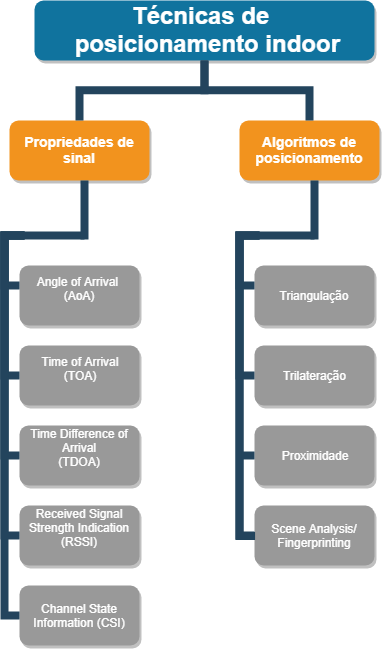
\includegraphics[scale = 0.4]{images/tecnicas_posicionamento_indoor.png}
	\caption{Técnicas localização indoor}
	\label{fig:tecnicas_posicionamento_indoor}
  \end{figure}


\subsection{Angle of Arrival}

Angle of Arrival (AoA), ou em português, ângulo de chegada é o angulo em que o sinal transmitido chega ao receptor. Abordagens baseadas no AoA, usam matrizes de antenas e exploram a diferença de fase das ondas recebidas em cada elemento dessa matriz. E com tal informação é possível estimar o AoA. Na figura \ref{fig:angle_of_arrival} mostra-se uma representação gráfica do processo.

Essa abordagem para estimativa do ângulo de chegada do sinal, geralmente envolve um hardware mais sofisticado quando em comparação com outras propriedades do sinal. Entretanto, com a informação do ângulo de chegada, algoritmos conseguem estimar uma localização com muito mais precisão.\cite{art2}

\begin{figure}[H]
	\centering 
	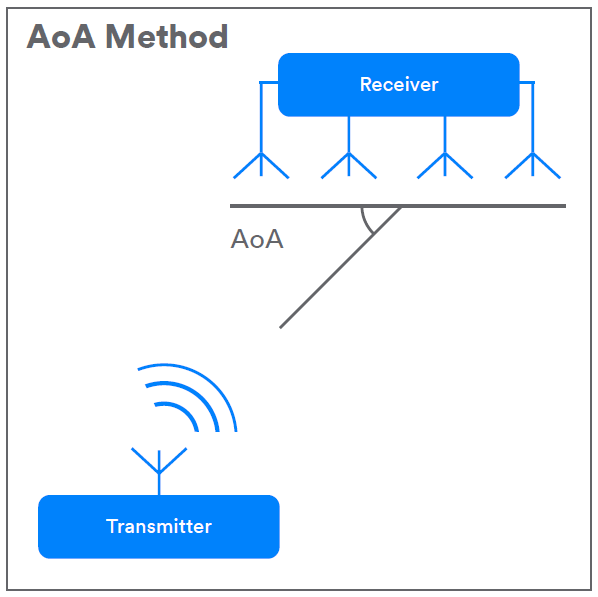
\includegraphics[scale = 0.6]{images/angle_of_arrival.png}
	\caption{Angle of Arrival (AoA)}
	\label{fig:angle_of_arrival}
\end{figure}

\subsection{Time of Arrival (ToA)}

Time of Arrival (ToA) também chamado de  Time of Flight (ToF) é uma técnica que explora o tempo transcorrido para o sinal emitido pelo transmissor chegar ao receptor. Multiplicando-se esse tempo pela velocidade de propagação da luz \(c = 3 \cdot 10^8\) é possível achar a distância entre o sinal recebido e o sinal transmitido. Entretanto essa técnica ainda não é muito precisa, devido as dimensões muito pequenas de tempo envolvidas em aplicaçãoes de curta distância \cite{art6}.

\subsection{Time Difference of Arrival (TDoA)}

Time Difference of Arrival (TDoA) se baseia na diferença nos tempos de propagação de diferentes transmissores, medidos em um receptor, se diferenciando do ToA em que o tempo absoluto é medido. Por essa razão sua complexidade é menor.
nesse método pelo menos 3 transmissores são necessários para determinar a localização do receptor resolvendo-se um conjunto de 3 equações de hipérboles \cite{art2}

\subsection{Received Signal Strength Indication (RSSI)}
Received Signal Strength Indication (RSSI) é a medida do nível de potência do sinal recebido em uma infraestrutura de radiofrequência e pode ser usado para estimação de distâncias.

Usando um modelo simples de propagação de perda de trajetória, a distância d entre transmissor e receptor pode ser estimada a partir de (5.1) como:

\begin{equation} \label{eq:rssi}
RSSI = -10n\log_{10} (d) + A 
\end{equation}

Em que n é o expoente de perda do ambiente (que varia de 2 em um espaço aberto a 4 em ambientes indoor) e A é o valor do RSSI em uma distância de referência do receptor

Entretanto, em ambientes indoor a medição do RSSI e o posicionamento podem ter suas precisões bem reduzidas. \cite{art1}

\subsection{Resumo}
Pode se contruir uma tabela indicando os principais aspectos dos métodos citados:

\begin{figure}[H]
	\centering 
	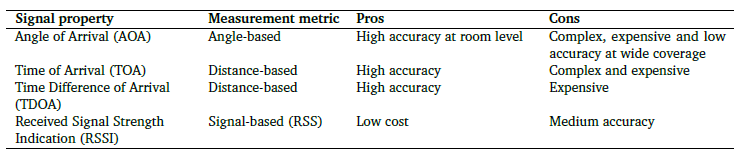
\includegraphics[scale = 1]{images/signal_table.png}
	\caption{Comparação entre técnicas de localização \cite{art1}}
	\label{fig:signal_table.png}
\end{figure}

\section{Algoritmos}

Algoritmos posicionais especificam como calcular a posição de um objeto alvo. Eles traduzem as propriedades dos sinais obtidos em distâncias e ângulos. Os principais algoritmos para localização atualmente são os de triangulação, trilateração, proximidade e o de \textit{scene analysis/fingerprinting}.

\subsection{Triangulação}
Triangulação usa as propriedades geométricas de triângulos para estimar a distância ao alvo por meio da computação de medidas angulares de dois pontos fixos de referência.
A posição de um objeto é encontrada na intercecção de dois pares de linhas de direção de ângulo.
Nesse caso, a propriedade de sinal que está diretamente envolvida é o AoA.

\subsection{Trilateração}
\label{sec:trilateracao}

A trilateração é um algoritmo para estimar a localização de posições desconhecidas baseado nas distâncias relativas para pontos conhecidos \cite{art12}.
Nesse método alguma propriedade do sinal fornece a distância relativa aos pontos conhecidos.

O processo pode ser exemplificado nas imagens abaixo em que as posições A, B e C são conhecidas e a D é desconhecida. Há 4 casos principais que podem acontecer dependendo das distâncias relativas obtidas:

\begin{enumerate}

	\item Circulos se interceptam em um único ponto:
	
	\begin{figure}[H]
		\centering 
		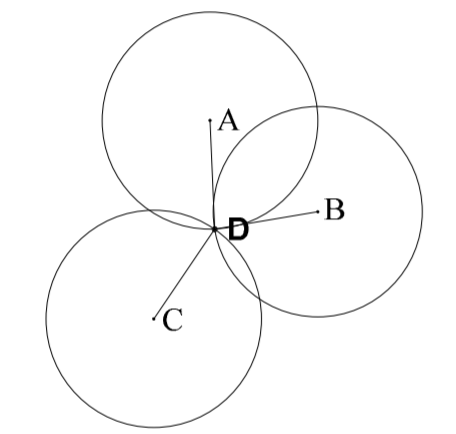
\includegraphics[scale = 1]{images/trilateration.png}
		\caption{Trilateração \cite{art12}}
		\label{fig:trilateration.png}
	\end{figure}
	
	
	As coordenadas podem ser denominadas de \( (x_n, y_n) \) em que n pode ser A, B, C ou D dependendo do ponto em questão. Dessa forma tem-se as seguintes equações:
	
	\begin{equation*}
	\begin{cases} \sqrt{(x - x_a)^2 + (y - y_a)^2} = d_a \\ \sqrt{(x - x_b)^2 + (y - y_b)^2} = d_b \\ \sqrt{(x - x_c)^2 + (y - y_c)^2} = d_c \end{cases}
	\end{equation*}
	
	Resolvendo-se a equação, obtém-se:
	
	\begin{equation*}
	\begin{bmatrix} 
		x \\
		y
	\end{bmatrix} = 
	\begin{bmatrix} 
		2(x_a - x_c) & 2(y_a - y_c) \\
		2(x_b - x_c) & 2(y_b - y_c)
	\end{bmatrix}^{-1}
	\begin{bmatrix} 
		x_a^2 - x_c^2 + y_a^2 - y_c^2 + d_c^2 - d_a^2 \\
		x_a^2 - x_c^2 + y_b^2 - y_c^2 + d_c^2 - d_b^2
	\end{bmatrix}
	\end{equation*}


\end{enumerate}	




\subsection{Proximidade}
É o algoritmo mais simples, entretanto só é utilizado para saber a distância de um objeto de interesse e não sua localização. Por tanto foge do escopo do presente trabalho.


\subsection{Scene analysis/fingerprinting}

Esses métodos se baseiam em coletar préviamente um conjunto de informações do sinal que são únicas a uma deteriminada localidade (\textit{fingerprint}) e posteriormente comparar com o \textit{fingerprint} do alvo. Com técnicas modernas de \textit{machine learning} é possivel encontrar padrões no \textit{fingerprint} de determinado sinal e comparar com posições armazenadas em um banco de dados que possuem \textit{fingerprints} similares \cite{art13}.

Algoritmos baseados nessa técnica são computacionalmente mais caros. Dessa forma o hardware se torna mais complexo. Mas por outro lado, grandes performances podem ser obtidas.

\subsection{Resumo}

Uma tabela pode ser construída comparando os principais pontos positivos e negativos de cada um desses algoritmos.
\begin{figure}[H]
	\centering 
	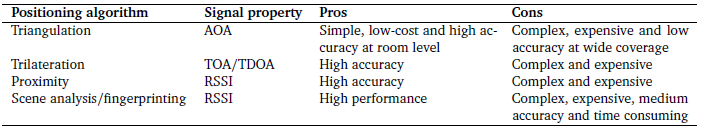
\includegraphics[scale = 1]{images/algorithms_table.png}
	\caption{Comparação entre algoritmos de localização \cite{art1}}
	\label{fig:algorithms_table.png}
\end{figure}

\section{Tecnologias para localização}
Diversas tecnologias têm-se mostrado úteis na função de localização indoor, porém cada um delas tem alguns aspectos positivos e negativos. A seguir se mostrará o estado-da-arte para cada tecnologia de localização. Os principais métodos se baseiam em radio-frequência (como Wi-Fi, Bluetooth, ZigBee, RFID e Ultra Wide Band ), entretanto métodos com luz, visível, ondas acústicas também podem ser utilizados.

\subsection{WiFi}
Wifi opera na banda ISM (Industrial, Scientific and Medical) utilizando principalmente a banda de 2.4GHz. É usada primariamente para a conexão com a internet e tem um alcance que pode chegar a 1Km. A maioria dos dispositivos portáteis são compatíveis com a tecnologia, assim soluções com Wifi não necessita grandes mudanças de infraestrutura. No entanto, interferências na banda ISM acabam afetando a precisão de localização. Além disso, não sendo o foco primário do WiFi a localização, mas sim a comunicação, faltam algoritmos eficientes para a localização.

Alguns trabalhos foram feitos demostrando as capacidades de localização com WiFi a exemplo de \cite{art7}

\subsection{Bluetooth}
Bluetooth é um padrão de tecnologia sem fio para trocar informação entre dispositivos móveis e fixos a curtas distancias. Usa ondas de rádio na banda ISM de 2.4 a 2.485GHz. Bluetooth Special Interest Group (SIG) é a organização responsável pelos padrões da tecnologia.

A última especificação do bluetooth, conhecida como Bluetooh 5.1 foi lançado em Janeiro de 2019, permite alcances de até 350m, velocidades de 2Mbit/s e possui baixo consumo energético \cite{art8}.

A maioria dos sistemas atuais de localização com bluetooth utilizam somente RSSI para estimar a posição, tais métodos atingem precisão entre 1m a 10m. Entretanto, a última especificação do Bluetooth, introduziu AoA, e testes iniciais mostram que a precisão para a localização utilizando algoritmos adequados pode chegar na ordem de centímetros \cite{art9}.

Outro ponto importante do Bluetooth é sua alta compatibilidade com dispositivos atuais. Devido a todos esses fatores, estima-se que até 2022 400 milhões de dispositivos de localização baseados em bluetooth sejam vendidos por ano \cite{art9}.

Um ponto negativo, é que o sinal de RSSI é reportado ao usuário com um intervalo de tempo grande, o que dificulta a localização em tempo real com tal tecnologia.

\subsection{ZigBee}

ZigBee é uma tecnologia sem fio desenhada para ser de baixo custo, ter baixa velocidade de dados e ter eficiência energética. Apesar de ser favorável para a localização em redes sem fio, não está disponível na maioria de dispositivos atuais, fazendo a tecnologia não ser favorável para localização indoor. \cite{art2}

\subsection{Ultra-Wideband (UWB)}
Ultra-wideband é uma tecnologia de comunicação que trabalha com bandas muito largas quando em comparação com outras tecnologias similares. As bandas passam de 500 MHZ. Tais bandas permitem uma série de vantagens como uma maior confiabilidade, ja que o sinal possui diversas componentes de frequência, o que aumenta a possibilidade de que pelo menos algumas passem por obstáculos \cite{art10}.
Além disso, devido aos pulsos de baixa duração (\(<\) 1ns) permitem métodos precisos de localização utilizando ToF, com precisão de centímetros. Desse modo é uma tecnologia promissora para a localização indoor.

Entretanto, o progresso lento do padrão de UWB tem limitado a adoção em larga escala da tecnologia.


\subsection{Sinais sonoros e ultrassônicos}

Utiliza-se sinais acústicos para a localização, de forma similar as tecnologias de radio-frequência.
A principal técnica utilizada é a de ToF, como as ondas de som se propagam a velocidades menores que as eletromagnéticas, tal método apresenta menores desafios em sua implementação. A precisão pode chegar na ordem de centímetros \cite{art11}.

Os maiores problemas são que na faixa audível potencias baixas tem que ser utilizadas para não causar uma poluição sonora. E a faixa audível é a com mais compatibilidade para microfones dos atuais \textit{smartphones}. Já para ondes ultrassônicas, o maior problema, consiste no fato de que a velocidade do som muda de acordo com a temperatura e umidade. Além disso, para ondas sonoras, sons ambientes podem causar uma grande interferência no sistema.


\subsection{Resumo}
A seguinte tabela foi tirada de \cite{art2} com um resumo dos principais pontos de cada tecnologia. Algumas tecnologias não foram citadas em detalhes no presente texto:

\begin{figure}[H]
	\centering 
	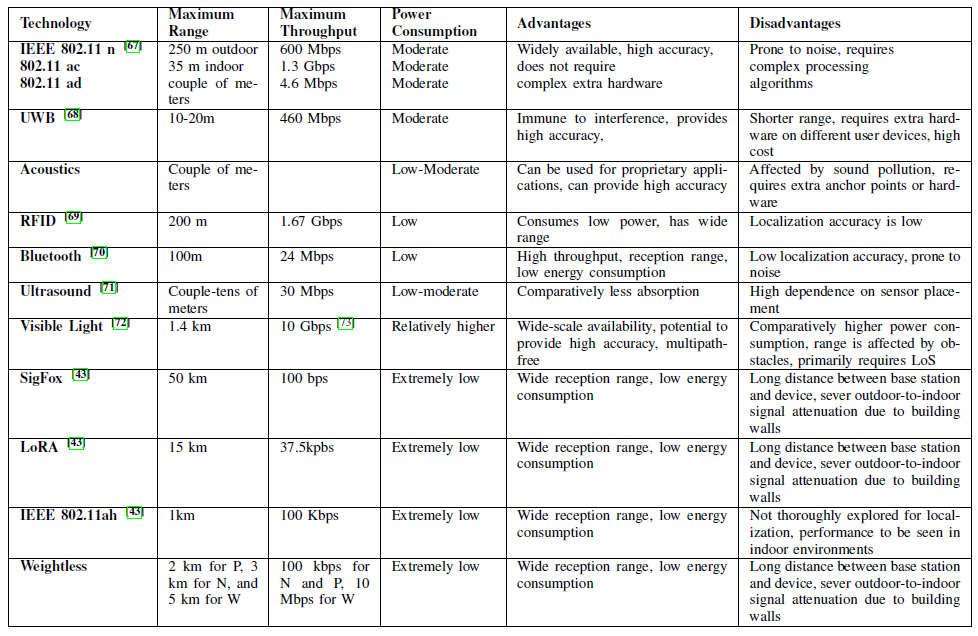
\includegraphics[scale = 0.7]{images/technologies_table.png}
	\caption{Comparação entre tecnologias possíveis para localização. Tirado de \cite{art2}}
	\label{fig:technologies_table}
\end{figure}
